\documentclass[1p]{elsarticle_modified}
%\bibliographystyle{elsarticle-num}

%\usepackage[colorlinks]{hyperref}
%\usepackage{abbrmath_seonhwa} %\Abb, \Ascr, \Acal ,\Abf, \Afrak
\usepackage{amsfonts}
\usepackage{amssymb}
\usepackage{amsmath}
\usepackage{amsthm}
\usepackage{scalefnt}
\usepackage{amsbsy}
\usepackage{kotex}
\usepackage{caption}
\usepackage{subfig}
\usepackage{color}
\usepackage{graphicx}
\usepackage{xcolor} %% white, black, red, green, blue, cyan, magenta, yellow
\usepackage{float}
\usepackage{setspace}
\usepackage{hyperref}

\usepackage{tikz}
\usetikzlibrary{arrows}

\usepackage{multirow}
\usepackage{array} % fixed length table
\usepackage{hhline}

%%%%%%%%%%%%%%%%%%%%%
\makeatletter
\renewcommand*\env@matrix[1][\arraystretch]{%
	\edef\arraystretch{#1}%
	\hskip -\arraycolsep
	\let\@ifnextchar\new@ifnextchar
	\array{*\c@MaxMatrixCols c}}
\makeatother %https://tex.stackexchange.com/questions/14071/how-can-i-increase-the-line-spacing-in-a-matrix
%%%%%%%%%%%%%%%

\usepackage[normalem]{ulem}

\newcommand{\msout}[1]{\ifmmode\text{\sout{\ensuremath{#1}}}\else\sout{#1}\fi}
%SOURCE: \msout is \stkout macro in https://tex.stackexchange.com/questions/20609/strikeout-in-math-mode

\newcommand{\cancel}[1]{
	\ifmmode
	{\color{red}\msout{#1}}
	\else
	{\color{red}\sout{#1}}
	\fi
}

\newcommand{\add}[1]{
	{\color{blue}\uwave{#1}}
}

\newcommand{\replace}[2]{
	\ifmmode
	{\color{red}\msout{#1}}{\color{blue}\uwave{#2}}
	\else
	{\color{red}\sout{#1}}{\color{blue}\uwave{#2}}
	\fi
}

\newcommand{\Sol}{\mathcal{S}} %segment
\newcommand{\D}{D} %diagram
\newcommand{\A}{\mathcal{A}} %arc


%%%%%%%%%%%%%%%%%%%%%%%%%%%%%5 test

\def\sl{\operatorname{\textup{SL}}(2,\Cbb)}
\def\psl{\operatorname{\textup{PSL}}(2,\Cbb)}
\def\quan{\mkern 1mu \triangleright \mkern 1mu}

\theoremstyle{definition}
\newtheorem{thm}{Theorem}[section]
\newtheorem{prop}[thm]{Proposition}
\newtheorem{lem}[thm]{Lemma}
\newtheorem{ques}[thm]{Question}
\newtheorem{cor}[thm]{Corollary}
\newtheorem{defn}[thm]{Definition}
\newtheorem{exam}[thm]{Example}
\newtheorem{rmk}[thm]{Remark}
\newtheorem{alg}[thm]{Algorithm}

\newcommand{\I}{\sqrt{-1}}
\begin{document}

%\begin{frontmatter}
%
%\title{Boundary parabolic representations of knots up to 8 crossings}
%
%%% Group authors per affiliation:
%\author{Yunhi Cho} 
%\address{Department of Mathematics, University of Seoul, Seoul, Korea}
%\ead{yhcho@uos.ac.kr}
%
%
%\author{Seonhwa Kim} %\fnref{s_kim}}
%\address{Center for Geometry and Physics, Institute for Basic Science, Pohang, 37673, Korea}
%\ead{ryeona17@ibs.re.kr}
%
%\author{Hyuk Kim}
%\address{Department of Mathematical Sciences, Seoul National University, Seoul 08826, Korea}
%\ead{hyukkim@snu.ac.kr}
%
%\author{Seokbeom Yoon}
%\address{Department of Mathematical Sciences, Seoul National University, Seoul, 08826,  Korea}
%\ead{sbyoon15@snu.ac.kr}
%
%\begin{abstract}
%We find all boundary parabolic representation of knots up to 8 crossings.
%
%\end{abstract}
%\begin{keyword}
%    \MSC[2010] 57M25 
%\end{keyword}
%
%\end{frontmatter}

%\linenumbers
%\tableofcontents
%
\newcommand\colored[1]{\textcolor{white}{\rule[-0.35ex]{0.8em}{1.4ex}}\kern-0.8em\color{red} #1}%
%\newcommand\colored[1]{\textcolor{white}{ #1}\kern-2.17ex	\textcolor{white}{ #1}\kern-1.81ex	\textcolor{white}{ #1}\kern-2.15ex\color{red}#1	}

{\Large $\underline{12a_{0200}~(K12a_{0200})}$}

\setlength{\tabcolsep}{10pt}
\renewcommand{\arraystretch}{1.6}
\vspace{1cm}\begin{tabular}{m{100pt}>{\centering\arraybackslash}m{274pt}}
\multirow{5}{120pt}{
	\centering
	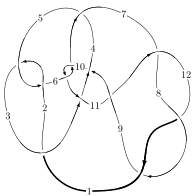
\includegraphics[width=112pt]{../../../GIT/diagram.site/Diagrams/png/1001_12a_0200.png}\\
\ \ \ A knot diagram\footnotemark}&
\allowdisplaybreaks
\textbf{Linearized knot diagam} \\
\cline{2-2}
 &
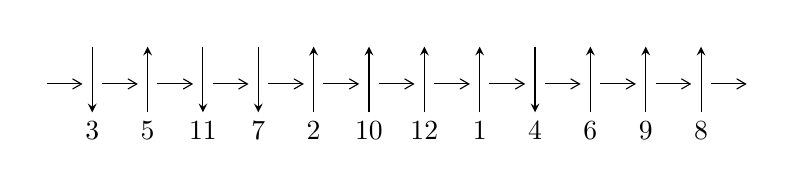
\begin{tikzpicture}[x=20pt, y=17pt]
	% nodes
	\node (C0) at (0, 0) {};
	\node (C1) at (1, 0) {};
	\node (C1U) at (1, +1) {};
	\node (C1D) at (1, -1) {3};

	\node (C2) at (2, 0) {};
	\node (C2U) at (2, +1) {};
	\node (C2D) at (2, -1) {5};

	\node (C3) at (3, 0) {};
	\node (C3U) at (3, +1) {};
	\node (C3D) at (3, -1) {11};

	\node (C4) at (4, 0) {};
	\node (C4U) at (4, +1) {};
	\node (C4D) at (4, -1) {7};

	\node (C5) at (5, 0) {};
	\node (C5U) at (5, +1) {};
	\node (C5D) at (5, -1) {2};

	\node (C6) at (6, 0) {};
	\node (C6U) at (6, +1) {};
	\node (C6D) at (6, -1) {10};

	\node (C7) at (7, 0) {};
	\node (C7U) at (7, +1) {};
	\node (C7D) at (7, -1) {12};

	\node (C8) at (8, 0) {};
	\node (C8U) at (8, +1) {};
	\node (C8D) at (8, -1) {1};

	\node (C9) at (9, 0) {};
	\node (C9U) at (9, +1) {};
	\node (C9D) at (9, -1) {4};

	\node (C10) at (10, 0) {};
	\node (C10U) at (10, +1) {};
	\node (C10D) at (10, -1) {6};

	\node (C11) at (11, 0) {};
	\node (C11U) at (11, +1) {};
	\node (C11D) at (11, -1) {9};

	\node (C12) at (12, 0) {};
	\node (C12U) at (12, +1) {};
	\node (C12D) at (12, -1) {8};
	\node (C13) at (13, 0) {};

	% arrows
	\draw[->,>={angle 60}]
	(C0) edge (C1) (C1) edge (C2) (C2) edge (C3) (C3) edge (C4) (C4) edge (C5) (C5) edge (C6) (C6) edge (C7) (C7) edge (C8) (C8) edge (C9) (C9) edge (C10) (C10) edge (C11) (C11) edge (C12) (C12) edge (C13) ;	\draw[->,>=stealth]
	(C1U) edge (C1D) (C2D) edge (C2U) (C3U) edge (C3D) (C4U) edge (C4D) (C5D) edge (C5U) (C6D) edge (C6U) (C7D) edge (C7U) (C8D) edge (C8U) (C9U) edge (C9D) (C10D) edge (C10U) (C11D) edge (C11U) (C12D) edge (C12U) ;
	\end{tikzpicture} \\
\hhline{~~} \\& 
\textbf{Solving Sequence} \\ \cline{2-2} 
 &
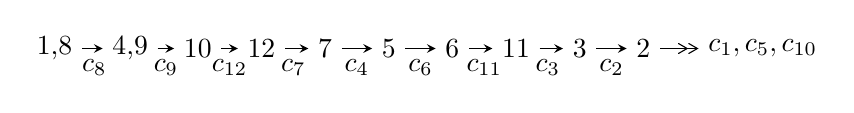
\begin{tikzpicture}[x=23pt, y=7pt]
	% node
	\node (A0) at (-1/8, 0) {1,8};
	\node (A1) at (17/16, 0) {4,9};
	\node (A2) at (17/8, 0) {10};
	\node (A3) at (25/8, 0) {12};
	\node (A4) at (33/8, 0) {7};
	\node (A5) at (41/8, 0) {5};
	\node (A6) at (49/8, 0) {6};
	\node (A7) at (57/8, 0) {11};
	\node (A8) at (65/8, 0) {3};
	\node (A9) at (73/8, 0) {2};
	\node (C1) at (1/2, -1) {$c_{8}$};
	\node (C2) at (13/8, -1) {$c_{9}$};
	\node (C3) at (21/8, -1) {$c_{12}$};
	\node (C4) at (29/8, -1) {$c_{7}$};
	\node (C5) at (37/8, -1) {$c_{4}$};
	\node (C6) at (45/8, -1) {$c_{6}$};
	\node (C7) at (53/8, -1) {$c_{11}$};
	\node (C8) at (61/8, -1) {$c_{3}$};
	\node (C9) at (69/8, -1) {$c_{2}$};
	\node (A10) at (11, 0) {$c_{1},c_{5},c_{10}$};

	% edge
	\draw[->,>=stealth]	
	(A0) edge (A1) (A1) edge (A2) (A2) edge (A3) (A3) edge (A4) (A4) edge (A5) (A5) edge (A6) (A6) edge (A7) (A7) edge (A8) (A8) edge (A9) ;
	\draw[->>,>={angle 60}]	
	(A9) edge (A10);
\end{tikzpicture} \\ 

\end{tabular} \\

\footnotetext{
The image of knot diagram is generated by the software ``\textbf{Draw programme}" developed by Andrew Bartholomew(\url{http://www.layer8.co.uk/maths/draw/index.htm\#Running-draw}), where we modified some parts for our purpose(\url{https://github.com/CATsTAILs/LinksPainter}).
}\phantom \\ \newline 
\centering \textbf{Ideals for irreducible components\footnotemark of $X_{\text{par}}$} 
 
\begin{align*}
I^u_{1}&=\langle 
-9.88128\times10^{122} u^{110}-1.62216\times10^{123} u^{109}+\cdots+3.02078\times10^{122} b-7.89614\times10^{122},\\
\phantom{I^u_{1}}&\phantom{= \langle  }2.57960\times10^{122} u^{110}+4.87705\times10^{121} u^{109}+\cdots+3.02078\times10^{122} a+1.07426\times10^{123},\\
\phantom{I^u_{1}}&\phantom{= \langle  }u^{111}+3 u^{110}+\cdots+8 u^2+1\rangle \\
I^u_{2}&=\langle 
a u+b+a,\;5 a^2+3 a u-4 a-3 u+5,\;u^2- u-1\rangle \\
\\
\end{align*}
\raggedright * 2 irreducible components of $\dim_{\mathbb{C}}=0$, with total 115 representations.\\
\footnotetext{All coefficients of polynomials are rational numbers. But the coefficients are sometimes approximated in decimal forms when there is not enough margin.}
\newpage
\renewcommand{\arraystretch}{1}
\centering \section*{I. $I^u_{1}= \langle -9.88\times10^{122} u^{110}-1.62\times10^{123} u^{109}+\cdots+3.02\times10^{122} b-7.90\times10^{122},\;2.58\times10^{122} u^{110}+4.88\times10^{121} u^{109}+\cdots+3.02\times10^{122} a+1.07\times10^{123},\;u^{111}+3 u^{110}+\cdots+8 u^2+1 \rangle$}
\flushleft \textbf{(i) Arc colorings}\\
\begin{tabular}{m{7pt} m{180pt} m{7pt} m{180pt} }
\flushright $a_{1}=$&$\begin{pmatrix}0\\u\end{pmatrix}$ \\
\flushright $a_{8}=$&$\begin{pmatrix}1\\0\end{pmatrix}$ \\
\flushright $a_{4}=$&$\begin{pmatrix}-0.853953 u^{110}-0.161450 u^{109}+\cdots+0.783670 u-3.55623\\3.27110 u^{110}+5.37000 u^{109}+\cdots-0.138489 u+2.61394\end{pmatrix}$ \\
\flushright $a_{9}=$&$\begin{pmatrix}1\\- u^2\end{pmatrix}$ \\
\flushright $a_{10}=$&$\begin{pmatrix}-0.971252 u^{110}-2.05773 u^{109}+\cdots+0.169491 u-2.13738\\2.96877 u^{110}+5.17690 u^{109}+\cdots-1.37894 u+2.55675\end{pmatrix}$ \\
\flushright $a_{12}=$&$\begin{pmatrix}- u\\u\end{pmatrix}$ \\
\flushright $a_{7}=$&$\begin{pmatrix}- u^2+1\\u^2\end{pmatrix}$ \\
\flushright $a_{5}=$&$\begin{pmatrix}0.852901 u^{110}+2.69009 u^{109}+\cdots-2.19989 u-2.77029\\0.859350 u^{110}+1.76075 u^{109}+\cdots+0.566412 u+1.25696\end{pmatrix}$ \\
\flushright $a_{6}=$&$\begin{pmatrix}-1.70072 u^{110}-2.81982 u^{109}+\cdots-2.03552 u-0.407690\\2.53069 u^{110}+3.23016 u^{109}+\cdots+0.436662 u+1.31110\end{pmatrix}$ \\
\flushright $a_{11}=$&$\begin{pmatrix}u^3-2 u\\- u^5+u^3+u\end{pmatrix}$ \\
\flushright $a_{3}=$&$\begin{pmatrix}0.828171 u^{110}+2.49944 u^{109}+\cdots-1.14740 u-2.51520\\0.699867 u^{110}+1.64618 u^{109}+\cdots+1.35387 u+1.06035\end{pmatrix}$ \\
\flushright $a_{2}=$&$\begin{pmatrix}-0.551106 u^{110}-1.46836 u^{109}+\cdots-6.95085 u-2.33008\\0.793459 u^{110}+1.82666 u^{109}+\cdots+2.35156 u+0.541040\end{pmatrix}$\\&\end{tabular}
\flushleft \textbf{(ii) Obstruction class $= -1$}\\~\\
\flushleft \textbf{(iii) Cusp Shapes $= 1.75758 u^{110}+2.71823 u^{109}+\cdots+4.75842 u+0.341861$}\\~\\
\newpage\renewcommand{\arraystretch}{1}
\flushleft \textbf{(iv) u-Polynomials at the component}\newline \\
\begin{tabular}{m{50pt}|m{274pt}}
Crossings & \hspace{64pt}u-Polynomials at each crossing \\
\hline $$\begin{aligned}c_{1}\end{aligned}$$&$\begin{aligned}
&u^{111}+49 u^{110}+\cdots+3796 u-625
\end{aligned}$\\
\hline $$\begin{aligned}c_{2},c_{5}\end{aligned}$$&$\begin{aligned}
&u^{111}+3 u^{110}+\cdots+314 u+25
\end{aligned}$\\
\hline $$\begin{aligned}c_{3}\end{aligned}$$&$\begin{aligned}
&25(25 u^{111}-35 u^{110}+\cdots+277470 u-25993)
\end{aligned}$\\
\hline $$\begin{aligned}c_{4}\end{aligned}$$&$\begin{aligned}
&25(25 u^{111}+70 u^{110}+\cdots-687 u-509)
\end{aligned}$\\
\hline $$\begin{aligned}c_{6},c_{10}\end{aligned}$$&$\begin{aligned}
&u^{111}-3 u^{110}+\cdots+2 u-1
\end{aligned}$\\
\hline $$\begin{aligned}c_{7},c_{8},c_{12}\end{aligned}$$&$\begin{aligned}
&u^{111}-3 u^{110}+\cdots-8 u^2-1
\end{aligned}$\\
\hline $$\begin{aligned}c_{9}\end{aligned}$$&$\begin{aligned}
&u^{111}- u^{110}+\cdots-5600 u-2000
\end{aligned}$\\
\hline $$\begin{aligned}c_{11}\end{aligned}$$&$\begin{aligned}
&u^{111}+9 u^{110}+\cdots+89858 u+4589
\end{aligned}$\\
\hline
\end{tabular}\\~\\
\newpage\renewcommand{\arraystretch}{1}
\flushleft \textbf{(v) Riley Polynomials at the component}\newline \\
\begin{tabular}{m{50pt}|m{274pt}}
Crossings & \hspace{64pt}Riley Polynomials at each crossing \\
\hline $$\begin{aligned}c_{1}\end{aligned}$$&$\begin{aligned}
&y^{111}+29 y^{110}+\cdots+12462116 y-390625
\end{aligned}$\\
\hline $$\begin{aligned}c_{2},c_{5}\end{aligned}$$&$\begin{aligned}
&y^{111}+49 y^{110}+\cdots+3796 y-625
\end{aligned}$\\
\hline $$\begin{aligned}c_{3}\end{aligned}$$&$\begin{aligned}
&625(625 y^{111}-10275 y^{110}+\cdots+4.35687\times10^{10} y-6.75636\times10^{8})
\end{aligned}$\\
\hline $$\begin{aligned}c_{4}\end{aligned}$$&$\begin{aligned}
&625(625 y^{111}-23850 y^{110}+\cdots-6.75091\times10^{7} y-259081)
\end{aligned}$\\
\hline $$\begin{aligned}c_{6},c_{10}\end{aligned}$$&$\begin{aligned}
&y^{111}+61 y^{110}+\cdots-16 y-1
\end{aligned}$\\
\hline $$\begin{aligned}c_{7},c_{8},c_{12}\end{aligned}$$&$\begin{aligned}
&y^{111}-99 y^{110}+\cdots-16 y-1
\end{aligned}$\\
\hline $$\begin{aligned}c_{9}\end{aligned}$$&$\begin{aligned}
&y^{111}-25 y^{110}+\cdots-12720000 y-4000000
\end{aligned}$\\
\hline $$\begin{aligned}c_{11}\end{aligned}$$&$\begin{aligned}
&y^{111}+9 y^{110}+\cdots+2636458452 y-21058921
\end{aligned}$\\
\hline
\end{tabular}\\~\\
\newpage\flushleft \textbf{(vi) Complex Volumes and Cusp Shapes}
$$\begin{array}{c|c|c}  
\text{Solutions to }I^u_{1}& \I (\text{vol} + \sqrt{-1}CS) & \text{Cusp shape}\\
 \hline 
\begin{aligned}
u &= -0.848451 + 0.533037 I \\
a &= -0.292158 + 0.517168 I \\
b &= \phantom{-}0.443974 - 0.962375 I\end{aligned}
 & \phantom{-}0.42545 + 3.75946 I & \phantom{-0.000000 } 0 \\ \hline\begin{aligned}
u &= -0.848451 - 0.533037 I \\
a &= -0.292158 - 0.517168 I \\
b &= \phantom{-}0.443974 + 0.962375 I\end{aligned}
 & \phantom{-}0.42545 - 3.75946 I & \phantom{-0.000000 } 0 \\ \hline\begin{aligned}
u &= \phantom{-}0.865725 + 0.468426 I \\
a &= \phantom{-}0.488857 + 0.754210 I \\
b &= -0.81665 - 1.59668 I\end{aligned}
 & -3.34824 - 9.97292 I & \phantom{-0.000000 } 0 \\ \hline\begin{aligned}
u &= \phantom{-}0.865725 - 0.468426 I \\
a &= \phantom{-}0.488857 - 0.754210 I \\
b &= -0.81665 + 1.59668 I\end{aligned}
 & -3.34824 + 9.97292 I & \phantom{-0.000000 } 0 \\ \hline\begin{aligned}
u &= \phantom{-}0.982269 + 0.291203 I \\
a &= -0.888257 + 0.097247 I \\
b &= \phantom{-}1.83582 + 0.03095 I\end{aligned}
 & -1.48534 + 4.18722 I & \phantom{-0.000000 } 0 \\ \hline\begin{aligned}
u &= \phantom{-}0.982269 - 0.291203 I \\
a &= -0.888257 - 0.097247 I \\
b &= \phantom{-}1.83582 - 0.03095 I\end{aligned}
 & -1.48534 - 4.18722 I & \phantom{-0.000000 } 0 \\ \hline\begin{aligned}
u &= -1.04175\phantom{ +0.000000I} \\
a &= \phantom{-}0.523490\phantom{ +0.000000I} \\
b &= -1.28841\phantom{ +0.000000I}\end{aligned}
 & \phantom{-}1.68448\phantom{ +0.000000I} & \phantom{-0.000000 } 0 \\ \hline\begin{aligned}
u &= \phantom{-}1.030970 + 0.293300 I \\
a &= \phantom{-}0.423550 + 0.949718 I \\
b &= -1.22150 - 1.85782 I\end{aligned}
 & -6.34532 - 1.55715 I & \phantom{-0.000000 } 0 \\ \hline\begin{aligned}
u &= \phantom{-}1.030970 - 0.293300 I \\
a &= \phantom{-}0.423550 - 0.949718 I \\
b &= -1.22150 + 1.85782 I\end{aligned}
 & -6.34532 + 1.55715 I & \phantom{-0.000000 } 0 \\ \hline\begin{aligned}
u &= \phantom{-}0.998551 + 0.450677 I \\
a &= \phantom{-}0.840429 + 0.185787 I \\
b &= -1.53447 - 0.47057 I\end{aligned}
 & -3.85932 + 8.71416 I & \phantom{-0.000000 } 0\\
 \hline 
 \end{array}$$\newpage$$\begin{array}{c|c|c}  
\text{Solutions to }I^u_{1}& \I (\text{vol} + \sqrt{-1}CS) & \text{Cusp shape}\\
 \hline 
\begin{aligned}
u &= \phantom{-}0.998551 - 0.450677 I \\
a &= \phantom{-}0.840429 - 0.185787 I \\
b &= -1.53447 + 0.47057 I\end{aligned}
 & -3.85932 - 8.71416 I & \phantom{-0.000000 } 0 \\ \hline\begin{aligned}
u &= \phantom{-}0.807023 + 0.379878 I \\
a &= -0.522999 - 0.820927 I \\
b &= \phantom{-}0.90293 + 1.46137 I\end{aligned}
 & -1.05540 - 4.59060 I & \phantom{-0.000000 } 0 \\ \hline\begin{aligned}
u &= \phantom{-}0.807023 - 0.379878 I \\
a &= -0.522999 + 0.820927 I \\
b &= \phantom{-}0.90293 - 1.46137 I\end{aligned}
 & -1.05540 + 4.59060 I & \phantom{-0.000000 } 0 \\ \hline\begin{aligned}
u &= \phantom{-}0.173431 + 0.853663 I \\
a &= -1.187460 - 0.697715 I \\
b &= -0.0829174 + 0.0476338 I\end{aligned}
 & -6.42513 - 4.06910 I & -4.22635 + 4.84629 I \\ \hline\begin{aligned}
u &= \phantom{-}0.173431 - 0.853663 I \\
a &= -1.187460 + 0.697715 I \\
b &= -0.0829174 - 0.0476338 I\end{aligned}
 & -6.42513 + 4.06910 I & -4.22635 - 4.84629 I \\ \hline\begin{aligned}
u &= -0.282130 + 0.822678 I \\
a &= \phantom{-}1.56370 + 0.05524 I \\
b &= -0.0108961 + 0.0640512 I\end{aligned}
 & -1.36655 - 8.48240 I & \phantom{-0.000000 -}0. + 8.35925 I \\ \hline\begin{aligned}
u &= -0.282130 - 0.822678 I \\
a &= \phantom{-}1.56370 - 0.05524 I \\
b &= -0.0108961 - 0.0640512 I\end{aligned}
 & -1.36655 + 8.48240 I & \phantom{-0.000000 } 0. - 8.35925 I \\ \hline\begin{aligned}
u &= \phantom{-}0.263131 + 0.807594 I \\
a &= -2.28540 + 0.02260 I \\
b &= -0.0613055 + 0.0463861 I\end{aligned}
 & -5.2649 + 14.5040 I & \phantom{-0.000000 } 0. - 9.52744 I \\ \hline\begin{aligned}
u &= \phantom{-}0.263131 - 0.807594 I \\
a &= -2.28540 - 0.02260 I \\
b &= -0.0613055 - 0.0463861 I\end{aligned}
 & -5.2649 - 14.5040 I & \phantom{-0.000000 -}0. + 9.52744 I \\ \hline\begin{aligned}
u &= \phantom{-}0.333797 + 0.766731 I \\
a &= -0.847130 - 0.808429 I \\
b &= \phantom{-}0.145580 + 0.030472 I\end{aligned}
 & -6.77766 + 2.81025 I & -4.73274 - 4.72373 I\\
 \hline 
 \end{array}$$\newpage$$\begin{array}{c|c|c}  
\text{Solutions to }I^u_{1}& \I (\text{vol} + \sqrt{-1}CS) & \text{Cusp shape}\\
 \hline 
\begin{aligned}
u &= \phantom{-}0.333797 - 0.766731 I \\
a &= -0.847130 + 0.808429 I \\
b &= \phantom{-}0.145580 - 0.030472 I\end{aligned}
 & -6.77766 - 2.81025 I & -4.73274 + 4.72373 I \\ \hline\begin{aligned}
u &= -0.678779 + 0.451474 I \\
a &= \phantom{-}0.128920 - 0.525934 I \\
b &= -0.306024 + 0.773797 I\end{aligned}
 & \phantom{-}1.90849 - 0.65389 I & \phantom{-}7.58705 + 0.13678 I \\ \hline\begin{aligned}
u &= -0.678779 - 0.451474 I \\
a &= \phantom{-}0.128920 + 0.525934 I \\
b &= -0.306024 - 0.773797 I\end{aligned}
 & \phantom{-}1.90849 + 0.65389 I & \phantom{-}7.58705 - 0.13678 I \\ \hline\begin{aligned}
u &= -1.120030 + 0.396848 I \\
a &= -0.447323 + 0.480647 I \\
b &= \phantom{-}0.88903 - 1.14435 I\end{aligned}
 & -1.02530 - 2.41413 I & \phantom{-0.000000 } 0 \\ \hline\begin{aligned}
u &= -1.120030 - 0.396848 I \\
a &= -0.447323 - 0.480647 I \\
b &= \phantom{-}0.88903 + 1.14435 I\end{aligned}
 & -1.02530 + 2.41413 I & \phantom{-0.000000 } 0 \\ \hline\begin{aligned}
u &= \phantom{-}0.255740 + 0.765219 I \\
a &= \phantom{-}2.44844 + 0.00182 I \\
b &= -0.0317545 - 0.0768044 I\end{aligned}
 & -2.89319 + 8.75711 I & \phantom{-}1.89232 - 6.34972 I \\ \hline\begin{aligned}
u &= \phantom{-}0.255740 - 0.765219 I \\
a &= \phantom{-}2.44844 - 0.00182 I \\
b &= -0.0317545 + 0.0768044 I\end{aligned}
 & -2.89319 - 8.75711 I & \phantom{-}1.89232 + 6.34972 I \\ \hline\begin{aligned}
u &= \phantom{-}0.668294 + 0.440594 I \\
a &= \phantom{-}0.381426 + 0.246199 I \\
b &= -0.946254 + 0.056017 I\end{aligned}
 & -5.52371 + 1.47662 I & -2.33166 - 2.56671 I \\ \hline\begin{aligned}
u &= \phantom{-}0.668294 - 0.440594 I \\
a &= \phantom{-}0.381426 - 0.246199 I \\
b &= -0.946254 - 0.056017 I\end{aligned}
 & -5.52371 - 1.47662 I & -2.33166 + 2.56671 I \\ \hline\begin{aligned}
u &= -0.279123 + 0.745093 I \\
a &= -1.66286 - 0.04574 I \\
b &= \phantom{-}0.0789298 - 0.0009419 I\end{aligned}
 & \phantom{-}0.44879 - 3.45366 I & \phantom{-}5.32609 + 3.91559 I\\
 \hline 
 \end{array}$$\newpage$$\begin{array}{c|c|c}  
\text{Solutions to }I^u_{1}& \I (\text{vol} + \sqrt{-1}CS) & \text{Cusp shape}\\
 \hline 
\begin{aligned}
u &= -0.279123 - 0.745093 I \\
a &= -1.66286 + 0.04574 I \\
b &= \phantom{-}0.0789298 + 0.0009419 I\end{aligned}
 & \phantom{-}0.44879 + 3.45366 I & \phantom{-}5.32609 - 3.91559 I \\ \hline\begin{aligned}
u &= -0.095794 + 0.780536 I \\
a &= \phantom{-}1.64142 + 0.32093 I \\
b &= \phantom{-}0.1096960 - 0.0870152 I\end{aligned}
 & -4.17950 - 1.81846 I & -2.32506 + 3.35231 I \\ \hline\begin{aligned}
u &= -0.095794 - 0.780536 I \\
a &= \phantom{-}1.64142 - 0.32093 I \\
b &= \phantom{-}0.1096960 + 0.0870152 I\end{aligned}
 & -4.17950 + 1.81846 I & -2.32506 - 3.35231 I \\ \hline\begin{aligned}
u &= -1.218480 + 0.084617 I \\
a &= \phantom{-}1.246560 - 0.353208 I \\
b &= -1.66716 - 0.71596 I\end{aligned}
 & -0.44945 + 3.45531 I & \phantom{-0.000000 } 0 \\ \hline\begin{aligned}
u &= -1.218480 - 0.084617 I \\
a &= \phantom{-}1.246560 + 0.353208 I \\
b &= -1.66716 + 0.71596 I\end{aligned}
 & -0.44945 - 3.45531 I & \phantom{-0.000000 } 0 \\ \hline\begin{aligned}
u &= \phantom{-}0.164141 + 0.752127 I \\
a &= -2.62610 + 0.40767 I \\
b &= \phantom{-}0.162415 - 0.114911 I\end{aligned}
 & -8.97208 + 5.45730 I & -4.50761 - 5.50179 I \\ \hline\begin{aligned}
u &= \phantom{-}0.164141 - 0.752127 I \\
a &= -2.62610 - 0.40767 I \\
b &= \phantom{-}0.162415 + 0.114911 I\end{aligned}
 & -8.97208 - 5.45730 I & -4.50761 + 5.50179 I \\ \hline\begin{aligned}
u &= -1.241840 + 0.229749 I \\
a &= -1.170840 - 0.281032 I \\
b &= \phantom{-}2.24935 - 0.85873 I\end{aligned}
 & \phantom{-}0.69363 - 1.61227 I & \phantom{-0.000000 } 0 \\ \hline\begin{aligned}
u &= -1.241840 - 0.229749 I \\
a &= -1.170840 + 0.281032 I \\
b &= \phantom{-}2.24935 + 0.85873 I\end{aligned}
 & \phantom{-}0.69363 + 1.61227 I & \phantom{-0.000000 } 0 \\ \hline\begin{aligned}
u &= \phantom{-}0.171856 + 0.716149 I \\
a &= \phantom{-}1.23312 + 1.09879 I \\
b &= \phantom{-}0.074081 + 0.131507 I\end{aligned}
 & -3.97774 - 0.39890 I & -0.933790 - 0.131410 I\\
 \hline 
 \end{array}$$\newpage$$\begin{array}{c|c|c}  
\text{Solutions to }I^u_{1}& \I (\text{vol} + \sqrt{-1}CS) & \text{Cusp shape}\\
 \hline 
\begin{aligned}
u &= \phantom{-}0.171856 - 0.716149 I \\
a &= \phantom{-}1.23312 - 1.09879 I \\
b &= \phantom{-}0.074081 - 0.131507 I\end{aligned}
 & -3.97774 + 0.39890 I & -0.933790 + 0.131410 I \\ \hline\begin{aligned}
u &= \phantom{-}1.263210 + 0.154487 I \\
a &= -0.77119 - 1.26137 I \\
b &= \phantom{-}0.90529 + 1.34726 I\end{aligned}
 & \phantom{-}2.59030 - 0.80985 I & \phantom{-0.000000 } 0 \\ \hline\begin{aligned}
u &= \phantom{-}1.263210 - 0.154487 I \\
a &= -0.77119 + 1.26137 I \\
b &= \phantom{-}0.90529 - 1.34726 I\end{aligned}
 & \phantom{-}2.59030 + 0.80985 I & \phantom{-0.000000 } 0 \\ \hline\begin{aligned}
u &= \phantom{-}1.306580 + 0.239131 I \\
a &= -2.36258 - 3.57462 I \\
b &= \phantom{-}1.74438 + 6.98773 I\end{aligned}
 & \phantom{-}1.22033 + 4.76626 I & \phantom{-0.000000 } 0 \\ \hline\begin{aligned}
u &= \phantom{-}1.306580 - 0.239131 I \\
a &= -2.36258 + 3.57462 I \\
b &= \phantom{-}1.74438 - 6.98773 I\end{aligned}
 & \phantom{-}1.22033 - 4.76626 I & \phantom{-0.000000 } 0 \\ \hline\begin{aligned}
u &= \phantom{-}1.332280 + 0.137029 I \\
a &= -1.26201 - 1.42638 I \\
b &= \phantom{-}3.20296 + 2.01883 I\end{aligned}
 & \phantom{-}3.35257 - 2.44507 I & \phantom{-0.000000 } 0 \\ \hline\begin{aligned}
u &= \phantom{-}1.332280 - 0.137029 I \\
a &= -1.26201 + 1.42638 I \\
b &= \phantom{-}3.20296 - 2.01883 I\end{aligned}
 & \phantom{-}3.35257 + 2.44507 I & \phantom{-0.000000 } 0 \\ \hline\begin{aligned}
u &= -0.172982 + 0.634595 I \\
a &= -0.36462 + 2.26997 I \\
b &= -0.012364 - 0.922385 I\end{aligned}
 & -3.15676 - 6.04076 I & -0.86742 + 10.32607 I \\ \hline\begin{aligned}
u &= -0.172982 - 0.634595 I \\
a &= -0.36462 - 2.26997 I \\
b &= -0.012364 + 0.922385 I\end{aligned}
 & -3.15676 + 6.04076 I & -0.86742 - 10.32607 I \\ \hline\begin{aligned}
u &= \phantom{-}1.329140 + 0.212562 I \\
a &= -0.98741 + 4.66926 I \\
b &= \phantom{-}4.54408 - 7.18236 I\end{aligned}
 & \phantom{-}1.33372 + 0.95736 I & \phantom{-0.000000 } 0\\
 \hline 
 \end{array}$$\newpage$$\begin{array}{c|c|c}  
\text{Solutions to }I^u_{1}& \I (\text{vol} + \sqrt{-1}CS) & \text{Cusp shape}\\
 \hline 
\begin{aligned}
u &= \phantom{-}1.329140 - 0.212562 I \\
a &= -0.98741 - 4.66926 I \\
b &= \phantom{-}4.54408 + 7.18236 I\end{aligned}
 & \phantom{-}1.33372 - 0.95736 I & \phantom{-0.000000 } 0 \\ \hline\begin{aligned}
u &= -0.038787 + 0.648227 I \\
a &= \phantom{-}2.76975 - 0.72668 I \\
b &= \phantom{-}0.949523 - 0.658677 I\end{aligned}
 & -2.97959 - 1.57809 I & \phantom{-}1.46253 + 6.32927 I \\ \hline\begin{aligned}
u &= -0.038787 - 0.648227 I \\
a &= \phantom{-}2.76975 + 0.72668 I \\
b &= \phantom{-}0.949523 + 0.658677 I\end{aligned}
 & -2.97959 + 1.57809 I & \phantom{-}1.46253 - 6.32927 I \\ \hline\begin{aligned}
u &= -1.341130 + 0.168721 I \\
a &= \phantom{-}0.836570 - 0.686707 I \\
b &= -2.39583 + 1.76770 I\end{aligned}
 & \phantom{-}4.84645 - 0.43250 I & \phantom{-0.000000 } 0 \\ \hline\begin{aligned}
u &= -1.341130 - 0.168721 I \\
a &= \phantom{-}0.836570 + 0.686707 I \\
b &= -2.39583 - 1.76770 I\end{aligned}
 & \phantom{-}4.84645 + 0.43250 I & \phantom{-0.000000 } 0 \\ \hline\begin{aligned}
u &= \phantom{-}1.323060 + 0.311518 I \\
a &= -1.23701 - 0.76718 I \\
b &= \phantom{-}2.21363 + 1.52328 I\end{aligned}
 & \phantom{-}0.26439 + 5.73172 I & \phantom{-0.000000 } 0 \\ \hline\begin{aligned}
u &= \phantom{-}1.323060 - 0.311518 I \\
a &= -1.23701 + 0.76718 I \\
b &= \phantom{-}2.21363 - 1.52328 I\end{aligned}
 & \phantom{-}0.26439 - 5.73172 I & \phantom{-0.000000 } 0 \\ \hline\begin{aligned}
u &= -1.349550 + 0.237179 I \\
a &= -0.353866 + 0.270005 I \\
b &= \phantom{-}1.45795 - 1.42502 I\end{aligned}
 & \phantom{-}3.91673 - 6.31648 I & \phantom{-0.000000 } 0 \\ \hline\begin{aligned}
u &= -1.349550 - 0.237179 I \\
a &= -0.353866 - 0.270005 I \\
b &= \phantom{-}1.45795 + 1.42502 I\end{aligned}
 & \phantom{-}3.91673 + 6.31648 I & \phantom{-0.000000 } 0 \\ \hline\begin{aligned}
u &= -1.359260 + 0.175859 I \\
a &= -0.295928 - 0.553147 I \\
b &= -0.46549 + 2.00688 I\end{aligned}
 & \phantom{-}5.30135 - 0.37795 I & \phantom{-0.000000 } 0\\
 \hline 
 \end{array}$$\newpage$$\begin{array}{c|c|c}  
\text{Solutions to }I^u_{1}& \I (\text{vol} + \sqrt{-1}CS) & \text{Cusp shape}\\
 \hline 
\begin{aligned}
u &= -1.359260 - 0.175859 I \\
a &= -0.295928 + 0.553147 I \\
b &= -0.46549 - 2.00688 I\end{aligned}
 & \phantom{-}5.30135 + 0.37795 I & \phantom{-0.000000 } 0 \\ \hline\begin{aligned}
u &= \phantom{-}1.364380 + 0.192376 I \\
a &= \phantom{-}1.090040 + 0.421563 I \\
b &= -1.79311 + 0.21609 I\end{aligned}
 & \phantom{-}5.58685 + 3.51795 I & \phantom{-0.000000 } 0 \\ \hline\begin{aligned}
u &= \phantom{-}1.364380 - 0.192376 I \\
a &= \phantom{-}1.090040 - 0.421563 I \\
b &= -1.79311 - 0.21609 I\end{aligned}
 & \phantom{-}5.58685 - 3.51795 I & \phantom{-0.000000 } 0 \\ \hline\begin{aligned}
u &= \phantom{-}1.363420 + 0.202853 I \\
a &= \phantom{-}1.25561 + 1.01262 I \\
b &= -2.57959 - 1.33084 I\end{aligned}
 & \phantom{-}5.45029 + 3.78361 I & \phantom{-0.000000 } 0 \\ \hline\begin{aligned}
u &= \phantom{-}1.363420 - 0.202853 I \\
a &= \phantom{-}1.25561 - 1.01262 I \\
b &= -2.57959 + 1.33084 I\end{aligned}
 & \phantom{-}5.45029 - 3.78361 I & \phantom{-0.000000 } 0 \\ \hline\begin{aligned}
u &= -1.365570 + 0.220575 I \\
a &= -1.02539 + 1.41423 I \\
b &= \phantom{-}2.90504 - 2.85866 I\end{aligned}
 & \phantom{-}4.69045 - 6.87284 I & \phantom{-0.000000 } 0 \\ \hline\begin{aligned}
u &= -1.365570 - 0.220575 I \\
a &= -1.02539 - 1.41423 I \\
b &= \phantom{-}2.90504 + 2.85866 I\end{aligned}
 & \phantom{-}4.69045 + 6.87284 I & \phantom{-0.000000 } 0 \\ \hline\begin{aligned}
u &= \phantom{-}1.360430 + 0.255439 I \\
a &= -1.067560 + 0.487762 I \\
b &= \phantom{-}1.34716 - 2.01980 I\end{aligned}
 & \phantom{-}1.69884 + 9.29683 I & \phantom{-0.000000 } 0 \\ \hline\begin{aligned}
u &= \phantom{-}1.360430 - 0.255439 I \\
a &= -1.067560 - 0.487762 I \\
b &= \phantom{-}1.34716 + 2.01980 I\end{aligned}
 & \phantom{-}1.69884 - 9.29683 I & \phantom{-0.000000 } 0 \\ \hline\begin{aligned}
u &= -1.367820 + 0.261256 I \\
a &= -0.296953 + 1.116880 I \\
b &= \phantom{-}0.34366 - 2.05651 I\end{aligned}
 & \phantom{-}0.88982 - 3.11273 I & \phantom{-0.000000 } 0\\
 \hline 
 \end{array}$$\newpage$$\begin{array}{c|c|c}  
\text{Solutions to }I^u_{1}& \I (\text{vol} + \sqrt{-1}CS) & \text{Cusp shape}\\
 \hline 
\begin{aligned}
u &= -1.367820 - 0.261256 I \\
a &= -0.296953 - 1.116880 I \\
b &= \phantom{-}0.34366 + 2.05651 I\end{aligned}
 & \phantom{-}0.88982 + 3.11273 I & \phantom{-0.000000 } 0 \\ \hline\begin{aligned}
u &= -1.358660 + 0.307497 I \\
a &= \phantom{-}1.47353 - 1.27627 I \\
b &= -3.02324 + 2.26120 I\end{aligned}
 & -4.16450 - 9.28584 I & \phantom{-0.000000 } 0 \\ \hline\begin{aligned}
u &= -1.358660 - 0.307497 I \\
a &= \phantom{-}1.47353 + 1.27627 I \\
b &= -3.02324 - 2.26120 I\end{aligned}
 & -4.16450 + 9.28584 I & \phantom{-0.000000 } 0 \\ \hline\begin{aligned}
u &= \phantom{-}0.131862 + 0.582545 I \\
a &= \phantom{-}1.70355 + 0.37972 I \\
b &= -0.055155 - 0.802252 I\end{aligned}
 & -0.78892 + 3.29378 I & \phantom{-}3.12146 - 3.00778 I \\ \hline\begin{aligned}
u &= \phantom{-}0.131862 - 0.582545 I \\
a &= \phantom{-}1.70355 - 0.37972 I \\
b &= -0.055155 + 0.802252 I\end{aligned}
 & -0.78892 - 3.29378 I & \phantom{-}3.12146 + 3.00778 I \\ \hline\begin{aligned}
u &= -1.355040 + 0.381279 I \\
a &= \phantom{-}0.383877 - 0.711688 I \\
b &= -0.76178 + 1.57252 I\end{aligned}
 & -1.62567 - 0.37101 I & \phantom{-0.000000 } 0 \\ \hline\begin{aligned}
u &= -1.355040 - 0.381279 I \\
a &= \phantom{-}0.383877 + 0.711688 I \\
b &= -0.76178 - 1.57252 I\end{aligned}
 & -1.62567 + 0.37101 I & \phantom{-0.000000 } 0 \\ \hline\begin{aligned}
u &= -1.40693 + 0.17203 I \\
a &= \phantom{-}0.268174 + 0.963385 I \\
b &= -0.422266 - 1.260740 I\end{aligned}
 & \phantom{-}0.77219 - 3.38057 I & \phantom{-0.000000 } 0 \\ \hline\begin{aligned}
u &= -1.40693 - 0.17203 I \\
a &= \phantom{-}0.268174 - 0.963385 I \\
b &= -0.422266 + 1.260740 I\end{aligned}
 & \phantom{-}0.77219 + 3.38057 I & \phantom{-0.000000 } 0 \\ \hline\begin{aligned}
u &= \phantom{-}0.199034 + 0.525414 I \\
a &= \phantom{-}3.35173 + 0.80061 I \\
b &= -0.535804 - 0.402837 I\end{aligned}
 & -0.26097 + 4.06974 I & \phantom{-}4.06125 - 10.23179 I\\
 \hline 
 \end{array}$$\newpage$$\begin{array}{c|c|c}  
\text{Solutions to }I^u_{1}& \I (\text{vol} + \sqrt{-1}CS) & \text{Cusp shape}\\
 \hline 
\begin{aligned}
u &= \phantom{-}0.199034 - 0.525414 I \\
a &= \phantom{-}3.35173 - 0.80061 I \\
b &= -0.535804 + 0.402837 I\end{aligned}
 & -0.26097 - 4.06974 I & \phantom{-}4.06125 + 10.23179 I \\ \hline\begin{aligned}
u &= -1.40718 + 0.30970 I \\
a &= -1.37279 + 1.25640 I \\
b &= \phantom{-}2.84341 - 2.55407 I\end{aligned}
 & \phantom{-}2.39755 - 12.65390 I & \phantom{-0.000000 } 0 \\ \hline\begin{aligned}
u &= -1.40718 - 0.30970 I \\
a &= -1.37279 - 1.25640 I \\
b &= \phantom{-}2.84341 + 2.55407 I\end{aligned}
 & \phantom{-}2.39755 + 12.65390 I & \phantom{-0.000000 } 0 \\ \hline\begin{aligned}
u &= -0.116165 + 0.546238 I \\
a &= -1.84090 + 2.69502 I \\
b &= -0.97453 + 1.07717 I\end{aligned}
 & -3.19745 + 1.83468 I & \phantom{-}5.65877 - 0.22358 I \\ \hline\begin{aligned}
u &= -0.116165 - 0.546238 I \\
a &= -1.84090 - 2.69502 I \\
b &= -0.97453 - 1.07717 I\end{aligned}
 & -3.19745 - 1.83468 I & \phantom{-}5.65877 + 0.22358 I \\ \hline\begin{aligned}
u &= \phantom{-}1.41464 + 0.30140 I \\
a &= \phantom{-}1.061040 + 0.878788 I \\
b &= -2.18989 - 1.69422 I\end{aligned}
 & \phantom{-}5.84224 + 7.26151 I & \phantom{-0.000000 } 0 \\ \hline\begin{aligned}
u &= \phantom{-}1.41464 - 0.30140 I \\
a &= \phantom{-}1.061040 - 0.878788 I \\
b &= -2.18989 + 1.69422 I\end{aligned}
 & \phantom{-}5.84224 - 7.26151 I & \phantom{-0.000000 } 0 \\ \hline\begin{aligned}
u &= -1.41616 + 0.32878 I \\
a &= \phantom{-}1.36309 - 1.23228 I \\
b &= -2.71714 + 2.56206 I\end{aligned}
 & \phantom{-}0.0783 - 18.6139 I & \phantom{-0.000000 } 0 \\ \hline\begin{aligned}
u &= -1.41616 - 0.32878 I \\
a &= \phantom{-}1.36309 + 1.23228 I \\
b &= -2.71714 - 2.56206 I\end{aligned}
 & \phantom{-}0.0783 + 18.6139 I & \phantom{-0.000000 } 0 \\ \hline\begin{aligned}
u &= \phantom{-}1.42537 + 0.33368 I \\
a &= -1.021320 - 0.833669 I \\
b &= \phantom{-}2.11056 + 1.70902 I\end{aligned}
 & \phantom{-}4.06837 + 12.66270 I & \phantom{-0.000000 } 0\\
 \hline 
 \end{array}$$\newpage$$\begin{array}{c|c|c}  
\text{Solutions to }I^u_{1}& \I (\text{vol} + \sqrt{-1}CS) & \text{Cusp shape}\\
 \hline 
\begin{aligned}
u &= \phantom{-}1.42537 - 0.33368 I \\
a &= -1.021320 + 0.833669 I \\
b &= \phantom{-}2.11056 - 1.70902 I\end{aligned}
 & \phantom{-}4.06837 - 12.66270 I & \phantom{-0.000000 } 0 \\ \hline\begin{aligned}
u &= -1.46504 + 0.04615 I \\
a &= -0.339493 + 0.294163 I \\
b &= -0.118355 + 0.261619 I\end{aligned}
 & \phantom{-}6.11070 + 3.64220 I & \phantom{-0.000000 } 0 \\ \hline\begin{aligned}
u &= -1.46504 - 0.04615 I \\
a &= -0.339493 - 0.294163 I \\
b &= -0.118355 - 0.261619 I\end{aligned}
 & \phantom{-}6.11070 - 3.64220 I & \phantom{-0.000000 } 0 \\ \hline\begin{aligned}
u &= -1.45238 + 0.31120 I \\
a &= \phantom{-}0.178801 - 0.780640 I \\
b &= -0.49079 + 1.48727 I\end{aligned}
 & -1.04831 - 6.74954 I & \phantom{-0.000000 } 0 \\ \hline\begin{aligned}
u &= -1.45238 - 0.31120 I \\
a &= \phantom{-}0.178801 + 0.780640 I \\
b &= -0.49079 - 1.48727 I\end{aligned}
 & -1.04831 + 6.74954 I & \phantom{-0.000000 } 0 \\ \hline\begin{aligned}
u &= -1.50530 + 0.01500 I \\
a &= \phantom{-}0.265699 - 0.377681 I \\
b &= \phantom{-}0.244666 + 0.006083 I\end{aligned}
 & \phantom{-}4.56452 + 9.01884 I & \phantom{-0.000000 } 0 \\ \hline\begin{aligned}
u &= -1.50530 - 0.01500 I \\
a &= \phantom{-}0.265699 + 0.377681 I \\
b &= \phantom{-}0.244666 - 0.006083 I\end{aligned}
 & \phantom{-}4.56452 - 9.01884 I & \phantom{-0.000000 } 0 \\ \hline\begin{aligned}
u &= -0.221727 + 0.438815 I \\
a &= -2.12355 - 0.19578 I \\
b &= \phantom{-}0.325288 + 0.377375 I\end{aligned}
 & \phantom{-}0.488487 - 1.269530 I & \phantom{-}6.63867 + 4.16913 I \\ \hline\begin{aligned}
u &= -0.221727 - 0.438815 I \\
a &= -2.12355 + 0.19578 I \\
b &= \phantom{-}0.325288 - 0.377375 I\end{aligned}
 & \phantom{-}0.488487 + 1.269530 I & \phantom{-}6.63867 - 4.16913 I \\ \hline\begin{aligned}
u &= -0.243843 + 0.413937 I \\
a &= -1.14024 - 1.03218 I \\
b &= \phantom{-}0.158306 + 0.677699 I\end{aligned}
 & \phantom{-}0.577620 - 1.139480 I & \phantom{-}7.59571 + 6.13511 I\\
 \hline 
 \end{array}$$\newpage$$\begin{array}{c|c|c}  
\text{Solutions to }I^u_{1}& \I (\text{vol} + \sqrt{-1}CS) & \text{Cusp shape}\\
 \hline 
\begin{aligned}
u &= -0.243843 - 0.413937 I \\
a &= -1.14024 + 1.03218 I \\
b &= \phantom{-}0.158306 - 0.677699 I\end{aligned}
 & \phantom{-}0.577620 + 1.139480 I & \phantom{-}7.59571 - 6.13511 I \\ \hline\begin{aligned}
u &= \phantom{-}1.51849 + 0.06536 I \\
a &= \phantom{-}0.149500 + 0.221635 I \\
b &= -0.095618 + 0.188264 I\end{aligned}
 & \phantom{-}9.19692 + 2.36753 I & \phantom{-0.000000 } 0 \\ \hline\begin{aligned}
u &= \phantom{-}1.51849 - 0.06536 I \\
a &= \phantom{-}0.149500 - 0.221635 I \\
b &= -0.095618 - 0.188264 I\end{aligned}
 & \phantom{-}9.19692 - 2.36753 I & \phantom{-0.000000 } 0 \\ \hline\begin{aligned}
u &= \phantom{-}0.261953 + 0.330905 I \\
a &= -1.54230 - 1.70626 I \\
b &= \phantom{-}0.557405 + 0.825682 I\end{aligned}
 & \phantom{-}0.32554 - 1.70816 I & \phantom{-}6.47908 + 1.51201 I \\ \hline\begin{aligned}
u &= \phantom{-}0.261953 - 0.330905 I \\
a &= -1.54230 + 1.70626 I \\
b &= \phantom{-}0.557405 - 0.825682 I\end{aligned}
 & \phantom{-}0.32554 + 1.70816 I & \phantom{-}6.47908 - 1.51201 I \\ \hline\begin{aligned}
u &= \phantom{-}1.61557 + 0.02903 I \\
a &= -0.0648338 - 0.0540396 I \\
b &= -0.089057 - 0.127793 I\end{aligned}
 & \phantom{-}8.92369 - 2.15451 I & \phantom{-0.000000 } 0 \\ \hline\begin{aligned}
u &= \phantom{-}1.61557 - 0.02903 I \\
a &= -0.0648338 + 0.0540396 I \\
b &= -0.089057 + 0.127793 I\end{aligned}
 & \phantom{-}8.92369 + 2.15451 I & \phantom{-0.000000 } 0 \\ \hline\begin{aligned}
u &= -0.362095 + 0.074063 I \\
a &= \phantom{-}2.75243 - 1.84793 I \\
b &= -0.834069 - 0.516392 I\end{aligned}
 & -1.43243 + 3.58403 I & \phantom{-}4.77704 - 2.61924 I \\ \hline\begin{aligned}
u &= -0.362095 - 0.074063 I \\
a &= \phantom{-}2.75243 + 1.84793 I \\
b &= -0.834069 + 0.516392 I\end{aligned}
 & -1.43243 - 3.58403 I & \phantom{-}4.77704 + 2.61924 I \\ \hline\begin{aligned}
u &= \phantom{-}0.166795 + 0.275988 I \\
a &= -2.86108 - 0.37335 I \\
b &= \phantom{-}0.432096 + 0.470414 I\end{aligned}
 & \phantom{-}0.19884 - 1.52275 I & \phantom{-}0.827561 + 0.763000 I\\
 \hline 
 \end{array}$$\newpage$$\begin{array}{c|c|c}  
\text{Solutions to }I^u_{1}& \I (\text{vol} + \sqrt{-1}CS) & \text{Cusp shape}\\
 \hline 
\begin{aligned}
u &= \phantom{-}0.166795 - 0.275988 I \\
a &= -2.86108 + 0.37335 I \\
b &= \phantom{-}0.432096 - 0.470414 I\end{aligned}
 & \phantom{-}0.19884 + 1.52275 I & \phantom{-}0.827561 - 0.763000 I\\
 \hline 
 \end{array}$$\newpage\newpage\renewcommand{\arraystretch}{1}
\centering \section*{II. $I^u_{2}= \langle a u+b+a,\;5 a^2+3 a u-4 a-3 u+5,\;u^2- u-1 \rangle$}
\flushleft \textbf{(i) Arc colorings}\\
\begin{tabular}{m{7pt} m{180pt} m{7pt} m{180pt} }
\flushright $a_{1}=$&$\begin{pmatrix}0\\u\end{pmatrix}$ \\
\flushright $a_{8}=$&$\begin{pmatrix}1\\0\end{pmatrix}$ \\
\flushright $a_{4}=$&$\begin{pmatrix}a\\- a u- a\end{pmatrix}$ \\
\flushright $a_{9}=$&$\begin{pmatrix}1\\- u-1\end{pmatrix}$ \\
\flushright $a_{10}=$&$\begin{pmatrix}1\\- u-1\end{pmatrix}$ \\
\flushright $a_{12}=$&$\begin{pmatrix}- u\\u\end{pmatrix}$ \\
\flushright $a_{7}=$&$\begin{pmatrix}- u\\u+1\end{pmatrix}$ \\
\flushright $a_{5}=$&$\begin{pmatrix}a u+2 a\\-3 a u-2 a\end{pmatrix}$ \\
\flushright $a_{6}=$&$\begin{pmatrix}0\\- u\end{pmatrix}$ \\
\flushright $a_{11}=$&$\begin{pmatrix}1\\-2 u-2\end{pmatrix}$ \\
\flushright $a_{3}=$&$\begin{pmatrix}a u+2 a\\-7 a u-5 a\end{pmatrix}$ \\
\flushright $a_{2}=$&$\begin{pmatrix}a u+2 a+u-1\\-7 a u-5 a-\frac{3}{5} u-\frac{1}{5}\end{pmatrix}$\\&\end{tabular}
\flushleft \textbf{(ii) Obstruction class $= 1$}\\~\\
\flushleft \textbf{(iii) Cusp Shapes $= \frac{387}{5} a u+\frac{259}{5} a+\frac{3}{5} u+5$}\\~\\
\newpage\renewcommand{\arraystretch}{1}
\flushleft \textbf{(iv) u-Polynomials at the component}\newline \\
\begin{tabular}{m{50pt}|m{274pt}}
Crossings & \hspace{64pt}u-Polynomials at each crossing \\
\hline $$\begin{aligned}c_{1},c_{5}\end{aligned}$$&$\begin{aligned}
&(u^2- u+1)^2
\end{aligned}$\\
\hline $$\begin{aligned}c_{2}\end{aligned}$$&$\begin{aligned}
&(u^2+u+1)^2
\end{aligned}$\\
\hline $$\begin{aligned}c_{3}\end{aligned}$$&$\begin{aligned}
&25(25 u^4+5 u^2+1)
\end{aligned}$\\
\hline $$\begin{aligned}c_{4}\end{aligned}$$&$\begin{aligned}
&25(25 u^4-25 u^3+20 u^2-5 u+1)
\end{aligned}$\\
\hline $$\begin{aligned}c_{6},c_{7},c_{8}\end{aligned}$$&$\begin{aligned}
&(u^2- u-1)^2
\end{aligned}$\\
\hline $$\begin{aligned}c_{9}\end{aligned}$$&$\begin{aligned}
&u^4
\end{aligned}$\\
\hline $$\begin{aligned}c_{10},c_{12}\end{aligned}$$&$\begin{aligned}
&(u^2+u-1)^2
\end{aligned}$\\
\hline $$\begin{aligned}c_{11}\end{aligned}$$&$\begin{aligned}
&(u^2-3 u+1)^2
\end{aligned}$\\
\hline
\end{tabular}\\~\\
\newpage\renewcommand{\arraystretch}{1}
\flushleft \textbf{(v) Riley Polynomials at the component}\newline \\
\begin{tabular}{m{50pt}|m{274pt}}
Crossings & \hspace{64pt}Riley Polynomials at each crossing \\
\hline $$\begin{aligned}c_{1},c_{2},c_{5}\end{aligned}$$&$\begin{aligned}
&(y^2+y+1)^2
\end{aligned}$\\
\hline $$\begin{aligned}c_{3}\end{aligned}$$&$\begin{aligned}
&625(25 y^2+5 y+1)^2
\end{aligned}$\\
\hline $$\begin{aligned}c_{4}\end{aligned}$$&$\begin{aligned}
&625(625 y^4+375 y^3+200 y^2+15 y+1)
\end{aligned}$\\
\hline $$\begin{aligned}c_{6},c_{7},c_{8}\\c_{10},c_{12}\end{aligned}$$&$\begin{aligned}
&(y^2-3 y+1)^2
\end{aligned}$\\
\hline $$\begin{aligned}c_{9}\end{aligned}$$&$\begin{aligned}
&y^4
\end{aligned}$\\
\hline $$\begin{aligned}c_{11}\end{aligned}$$&$\begin{aligned}
&(y^2-7 y+1)^2
\end{aligned}$\\
\hline
\end{tabular}\\~\\
\newpage\flushleft \textbf{(vi) Complex Volumes and Cusp Shapes}
$$\begin{array}{c|c|c}  
\text{Solutions to }I^u_{2}& \I (\text{vol} + \sqrt{-1}CS) & \text{Cusp shape}\\
 \hline 
\begin{aligned}
u &= -0.618034\phantom{ +0.000000I} \\
a &= \phantom{-}0.585410 + 1.013960 I \\
b &= -0.223607 - 0.387298 I\end{aligned}
 & \phantom{-}0.98696 - 2.02988 I & \phantom{-}6.94984 + 4.01951 I \\ \hline\begin{aligned}
u &= -0.618034\phantom{ +0.000000I} \\
a &= \phantom{-}0.585410 - 1.013960 I \\
b &= -0.223607 + 0.387298 I\end{aligned}
 & \phantom{-}0.98696 + 2.02988 I & \phantom{-}6.94984 - 4.01951 I \\ \hline\begin{aligned}
u &= \phantom{-}1.61803\phantom{ +0.000000I} \\
a &= -0.085410 + 0.147935 I \\
b &= \phantom{-}0.223607 - 0.387298 I\end{aligned}
 & \phantom{-}8.88264 + 2.02988 I & -9.1498 + 26.1898 I \\ \hline\begin{aligned}
u &= \phantom{-}1.61803\phantom{ +0.000000I} \\
a &= -0.085410 - 0.147935 I \\
b &= \phantom{-}0.223607 + 0.387298 I\end{aligned}
 & \phantom{-}8.88264 - 2.02988 I & -9.1498 - 26.1898 I\\
 \hline 
 \end{array}$$\newpage
\newpage\renewcommand{\arraystretch}{1}
\centering \section*{ III. u-Polynomials}
\begin{tabular}{m{50pt}|m{274pt}}
Crossings & \hspace{64pt}u-Polynomials at each crossing \\
\hline $$\begin{aligned}c_{1}\end{aligned}$$&$\begin{aligned}
&((u^2- u+1)^2)(u^{111}+49 u^{110}+\cdots+3796 u-625)
\end{aligned}$\\
\hline $$\begin{aligned}c_{2}\end{aligned}$$&$\begin{aligned}
&((u^2+u+1)^2)(u^{111}+3 u^{110}+\cdots+314 u+25)
\end{aligned}$\\
\hline $$\begin{aligned}c_{3}\end{aligned}$$&$\begin{aligned}
&625(25 u^4+5 u^2+1)(25 u^{111}-35 u^{110}+\cdots+277470 u-25993)
\end{aligned}$\\
\hline $$\begin{aligned}c_{4}\end{aligned}$$&$\begin{aligned}
&625(25 u^4-25 u^3+\cdots-5 u+1)(25 u^{111}+70 u^{110}+\cdots-687 u-509)
\end{aligned}$\\
\hline $$\begin{aligned}c_{5}\end{aligned}$$&$\begin{aligned}
&((u^2- u+1)^2)(u^{111}+3 u^{110}+\cdots+314 u+25)
\end{aligned}$\\
\hline $$\begin{aligned}c_{6}\end{aligned}$$&$\begin{aligned}
&((u^2- u-1)^2)(u^{111}-3 u^{110}+\cdots+2 u-1)
\end{aligned}$\\
\hline $$\begin{aligned}c_{7},c_{8}\end{aligned}$$&$\begin{aligned}
&((u^2- u-1)^2)(u^{111}-3 u^{110}+\cdots-8 u^2-1)
\end{aligned}$\\
\hline $$\begin{aligned}c_{9}\end{aligned}$$&$\begin{aligned}
&u^4(u^{111}- u^{110}+\cdots-5600 u-2000)
\end{aligned}$\\
\hline $$\begin{aligned}c_{10}\end{aligned}$$&$\begin{aligned}
&((u^2+u-1)^2)(u^{111}-3 u^{110}+\cdots+2 u-1)
\end{aligned}$\\
\hline $$\begin{aligned}c_{11}\end{aligned}$$&$\begin{aligned}
&((u^2-3 u+1)^2)(u^{111}+9 u^{110}+\cdots+89858 u+4589)
\end{aligned}$\\
\hline $$\begin{aligned}c_{12}\end{aligned}$$&$\begin{aligned}
&((u^2+u-1)^2)(u^{111}-3 u^{110}+\cdots-8 u^2-1)
\end{aligned}$\\
\hline
\end{tabular}\newpage\renewcommand{\arraystretch}{1}
\centering \section*{ IV. Riley Polynomials}
\begin{tabular}{m{50pt}|m{274pt}}
Crossings & \hspace{64pt}Riley Polynomials at each crossing \\
\hline $$\begin{aligned}c_{1}\end{aligned}$$&$\begin{aligned}
&((y^2+y+1)^2)(y^{111}+29 y^{110}+\cdots+1.24621\times10^{7} y-390625)
\end{aligned}$\\
\hline $$\begin{aligned}c_{2},c_{5}\end{aligned}$$&$\begin{aligned}
&((y^2+y+1)^2)(y^{111}+49 y^{110}+\cdots+3796 y-625)
\end{aligned}$\\
\hline $$\begin{aligned}c_{3}\end{aligned}$$&$\begin{aligned}
&390625(25 y^2+5 y+1)^2\\
&\cdot(625 y^{111}-10275 y^{110}+\cdots+43568737248 y-675636049)
\end{aligned}$\\
\hline $$\begin{aligned}c_{4}\end{aligned}$$&$\begin{aligned}
&390625(625 y^4+375 y^3+200 y^2+15 y+1)\\
&\cdot(625 y^{111}-23850 y^{110}+\cdots-67509053 y-259081)
\end{aligned}$\\
\hline $$\begin{aligned}c_{6},c_{10}\end{aligned}$$&$\begin{aligned}
&((y^2-3 y+1)^2)(y^{111}+61 y^{110}+\cdots-16 y-1)
\end{aligned}$\\
\hline $$\begin{aligned}c_{7},c_{8},c_{12}\end{aligned}$$&$\begin{aligned}
&((y^2-3 y+1)^2)(y^{111}-99 y^{110}+\cdots-16 y-1)
\end{aligned}$\\
\hline $$\begin{aligned}c_{9}\end{aligned}$$&$\begin{aligned}
&y^4(y^{111}-25 y^{110}+\cdots-1.27200\times10^{7} y-4000000)
\end{aligned}$\\
\hline $$\begin{aligned}c_{11}\end{aligned}$$&$\begin{aligned}
&((y^2-7 y+1)^2)(y^{111}+9 y^{110}+\cdots+2.63646\times10^{9} y-2.10589\times10^{7})
\end{aligned}$\\
\hline
\end{tabular}
\vskip 2pc
\end{document}